\section{Validierung}\label{sec:Validierung}
In diesem Kapitel wird zuerst der Versuchsaufbau erklärt. Danach werden die einzelnen Versuche und deren Erkenntnis erläutert.

\subsection{Versuchsaufbau}\label{subsec:Versuchsaufbau}
Für den Versuchsaufbau wurde BLDC-Motor mit einer asynchronen Maschine gekoppelt welche über einen Frequenzumrichter angesteuert wird. Die asynchrone Maschine dient bei diesen Versuche als Last.


\subsection{Drehmoment bei variabler Drehzahl}\label{subsec:DrehmomentDrehzahl}
Bei diesem ersten Versuch gilt es zu verifizieren, ob der BLDC-Motor das erforderliche Drehmoment unabhängig von der Drehzahl erreichen kann.

% dieser Teil eventulle in den Hartwareteil verschieben und nur darauf Referenzieren
Bei einem minimalen mechanischen Wirkungsgrad von 0.8, einem 1:16 Getriebe und einem Trommeldurchmesser von 80cm, muss der Motor ein konstantes Drehmoment von 32Nm liefern.

Das Drehmoment an der Welle des BLDC-Motors wird mithilfe der Formel (FORMEL IN HARWARE/GRUNDLAGEN) über die Leistung und der Drehzahl des Motors ermittelt. Diese Kurve ist in der Abbildung \ref{fig:drehmoment/drehzahl} (blaue Kurve) ersichtlich. Da die asynchrone Maschine ebenfalls nicht ideal arbeitet, wird bei dieser einen Wirkungsgrad von 90\% angenommen (rote Kurve). 

\begin{figure}[H]
	\centering
	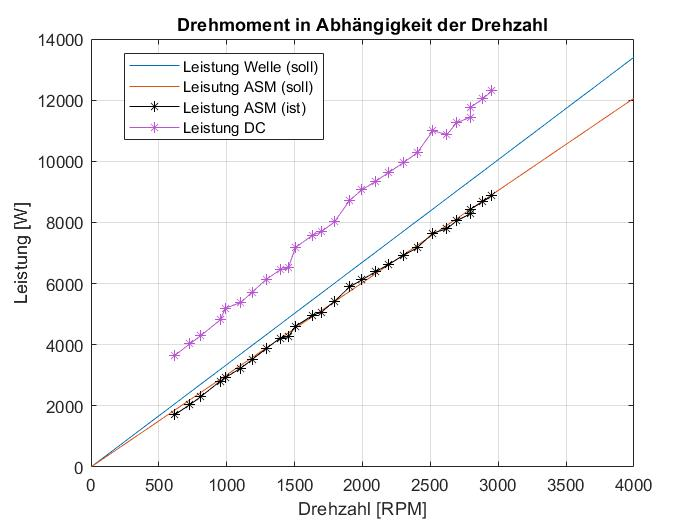
\includegraphics[width=0.8\linewidth]{drehmoment_drehzahl.jpg}
	\caption{Drehmoment in Abhängigkeit der Drehzahl}\label{fig:drehmoment/drehzahl}
\end{figure}

Bei diesem Versuch ist ersichtlich, dass es möglich war, die erforderliche Leistung (schwarze Punkte) im Drehzahlbereich zwischen 600 und 3000 RPM zu erreichen. Die aufgenommene Leistung auf der DC-Seite (violette Punkte) ist dabei proportional zur abgegebenen Leistung angestiegen.

In der Abbildung \ref{fig:drehmoment/StromSpannung} sind die Spannung, der Strom und die Sollwertvorgabe für die Ansteuerung während des Versuchs ersichtlich. Die Spannung wurde nachgeregelt (blaue Punkte), damit diese konstant bleibt. Der Strom (rote Punkte) und der Sollwert für die Ansteuerung (orange Punkte) wurden ebenfalls während des Versuchs dokumentiert.

\begin{figure}[H]
	\centering
	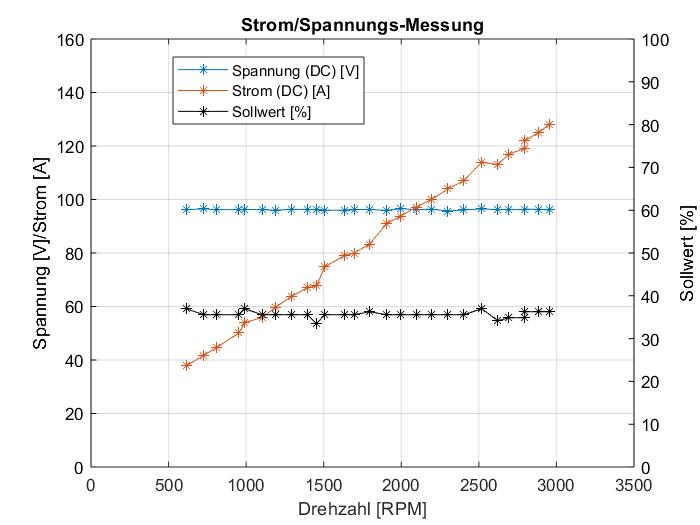
\includegraphics[width=0.8\linewidth]{drehmoment_StromSpannung.jpg}
	\caption{Spannung und Strom während des Drehmomentversuchs}\label{fig:drehmoment/StromSpannung}
\end{figure}

Da der graue Transformator nur für einen Strom von 95A konzipiert ist, was einem Strom von ca. 128A im DC-Zwischenkreis entspricht, konnte der Versuch nicht bis 3800 RPM durchgeführt werden. Der Strom kann mit guter Näherung als linear zur Drehzahl bei gleichbleibendem Drehmoment betrachtet werden. Dadurch ist ersichtlich, dass bei 3800 RPM ein Strom von ca. 160A benötigt wird. Dies Stromstärke deckt sich auch mit dem, was im Datenblatt des Motors angegeben wird (REFERENZ AUF DATENBLATT).

Bei diesem Versuch ist ebenfalls ersichtlich, dass die Sollwertvorgabe über den Drehzahlbereich nur kleine Abweichungen hat und daher in guter Näherung als konstant betrachtet werden kann.


\subsection{Leistungsverhalten bei Spannungsabfall}\label{subsec:LeistungSpannungabfall}
Bei diesem Versuch wird das Verhalten des Controllers bei einem Spannungsabfall untersucht. Dabei wurde die Leistung der asynchronen Maschine (rechte Abbildung) und der Strom (linke Abbildung) des Controllers in Abhängigkeit der Spannung des Controllers gemessen. Der Sollwert wurde während des gesamten Versuchs konstant auf 35.5\% gehalten, was dem Wert des Drehmomentversuchs entspricht. Dieser Versuch wurde zuerst mit 1500 RPM (blaue Punkte) und danach nochmals mit 2000 RPM (rote Punkte) durchgeführt.

\begin{figure}[H]
	\centering
	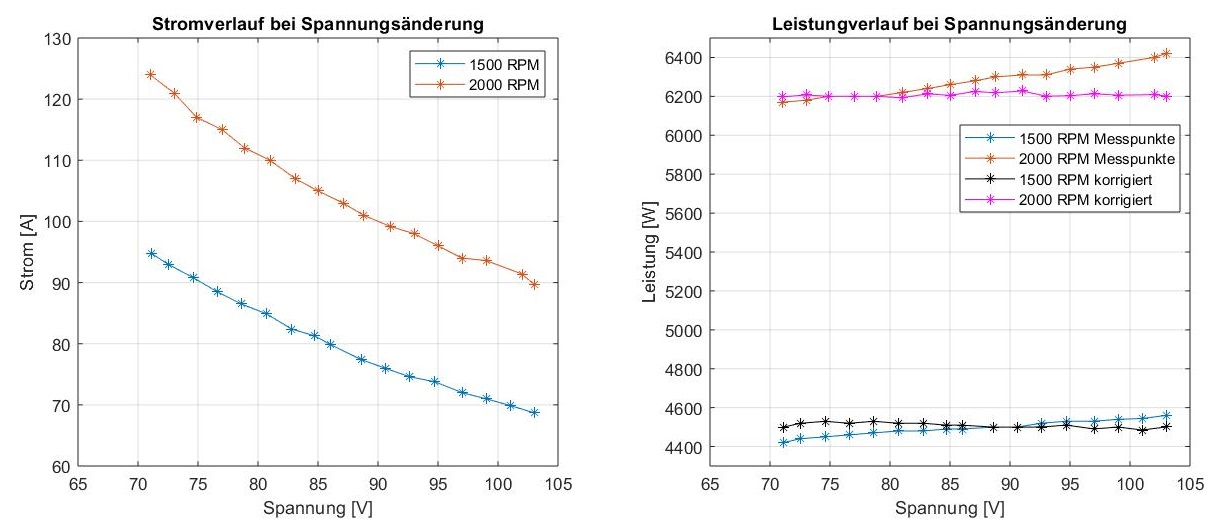
\includegraphics[width=1\linewidth]{Spannungsversuch.jpg}
	\caption{Leistungs- und Stromverlauf bei Spannungsabfall}\label{fig:Spannungsabfall}
\end{figure}

Aus diesem Versuch ist ersichtlich, dass der Controller bei einem Spannungsabfall und konstantem Drehmomentsollwert die Leistung nachregelt indem der Strom erhöht wird. Während die Spannung um 32\% abfällt, nimmt der Strom um ca. 28\% zu. Dabei verhält sich die Stromzunahme linear zum Spannungsabfall. Die Leistung nimmt dabei lediglich um ca. 4\% ab.

Dadurch kann der Schluss gezogen werden, dass der Spannungsabfall keinen grossen Einfluss auf die Leistung hat. Durch die erhöhte thermische Belastung bei grösseren Ströme ist eine möglichst grosse Spannung jedoch erstrebenswert.

\subsection{Maximale Drehzahl bei variabler Spannung}\label{subsec:DrehzahlSpanungsabfall}
In diesem Versuch wird das Verhalten des Motors bei Unterspannung untersucht. Dabei wurde der Sollwert für das Drehmoment auf dem Maximum gehalten, während der Motor im Leerlauf dreht. Die Spannung wird dabei langsam erhöht. Die Drehzahl ist dabei elektronisch im Controller auf 3800 RPM begrenzt, da die asynchrone Maschine keine höheren Drehzahlen zulässt.

\begin{figure}[H]
	\centering
	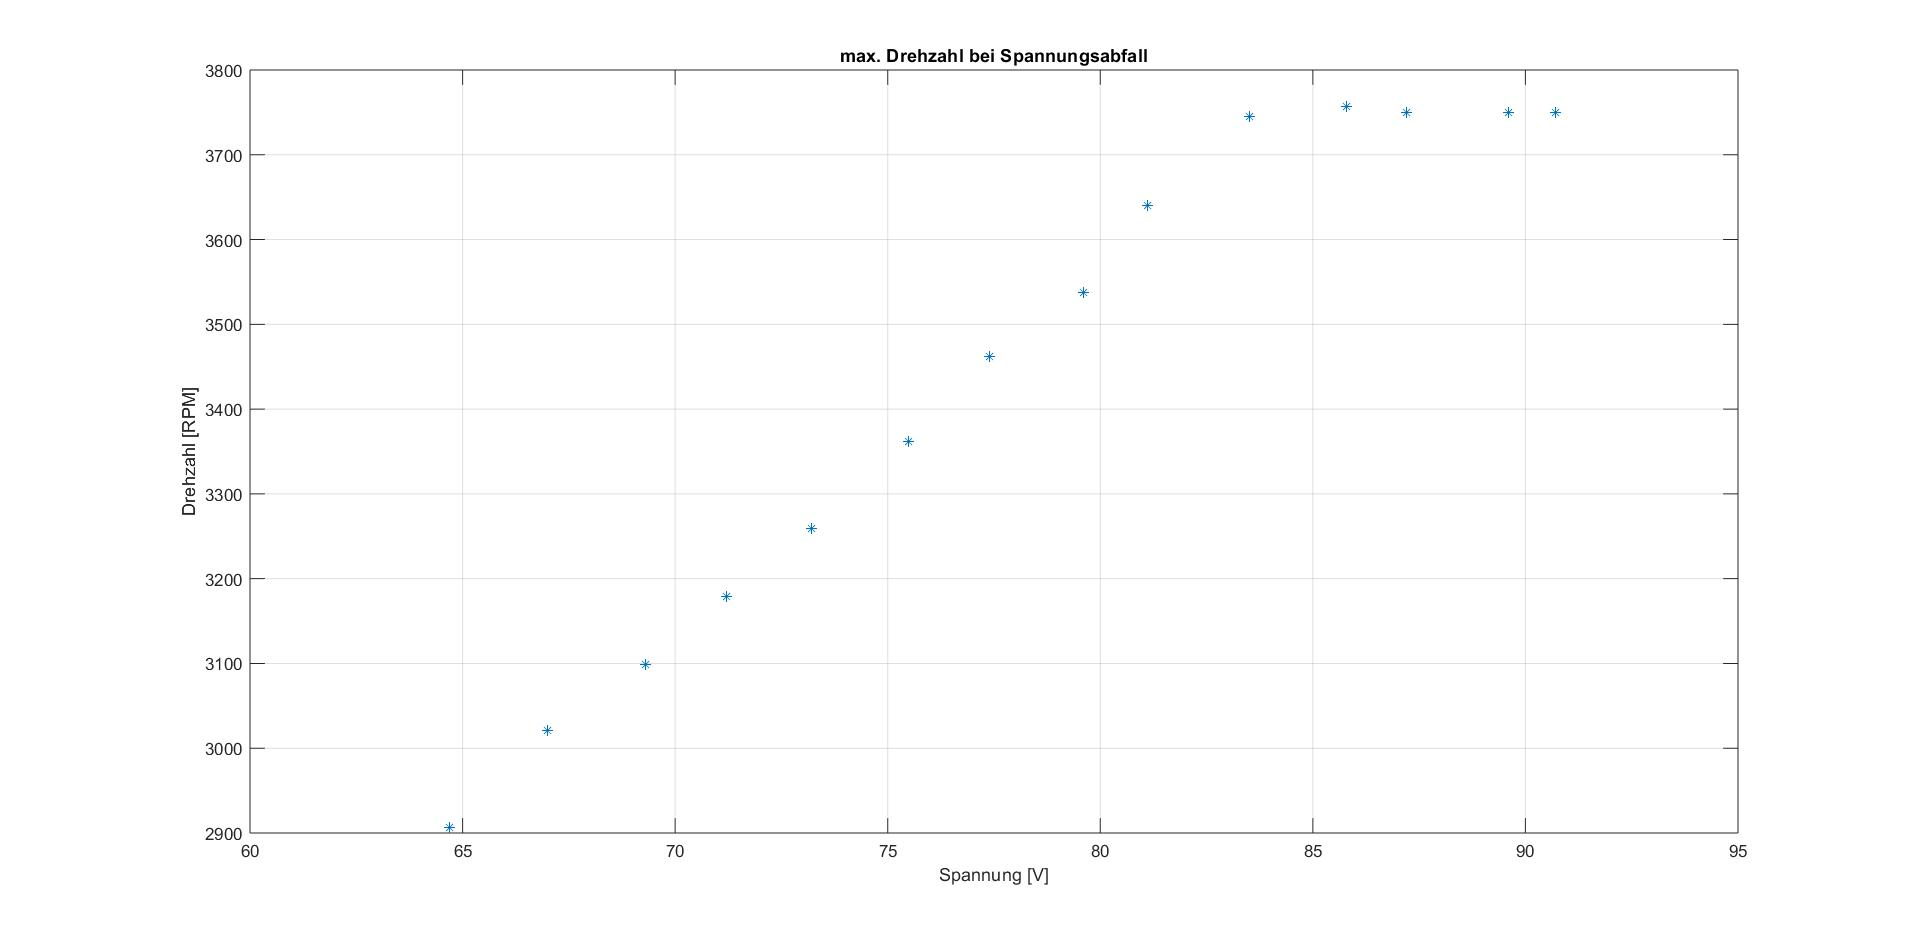
\includegraphics[width=0.8\linewidth]{maxDrehzahl.jpg}
	\caption{Maximale Drehzahl}\label{fig:maxDrehzahl}
\end{figure}

Bei diesem Versuch hat sich gezeigt, dass die Versorgung mindestens 84V bringen muss, damit der BLDC-Motor 3800 RPM erreichen kann. Weiter ist ersichtlich, dass die Leerlaufdrehzahl ca. 45 RPM pro Volt sinkt.


\subsection{Maximale Leistung bei variabler Spannung}\label{subsec:LeistungSpannungsabfall}
In diesem Versuch wird die maximale Leistung bei einem Spannungsabfall untersucht. Da die asynchrone Maschine nicht für 3800 RPM ausgelegt ist, wurde dieser Versuch bei einer konstanten Drehzahl von 3600 RPM gemessen. Dabei wurde, wie im vorhergehenden Versuch, das Drehmoment wieder auf das Maximum gesetzt, während die Spannung langsam erhöht wird.


\begin{figure}[H]
	\centering
	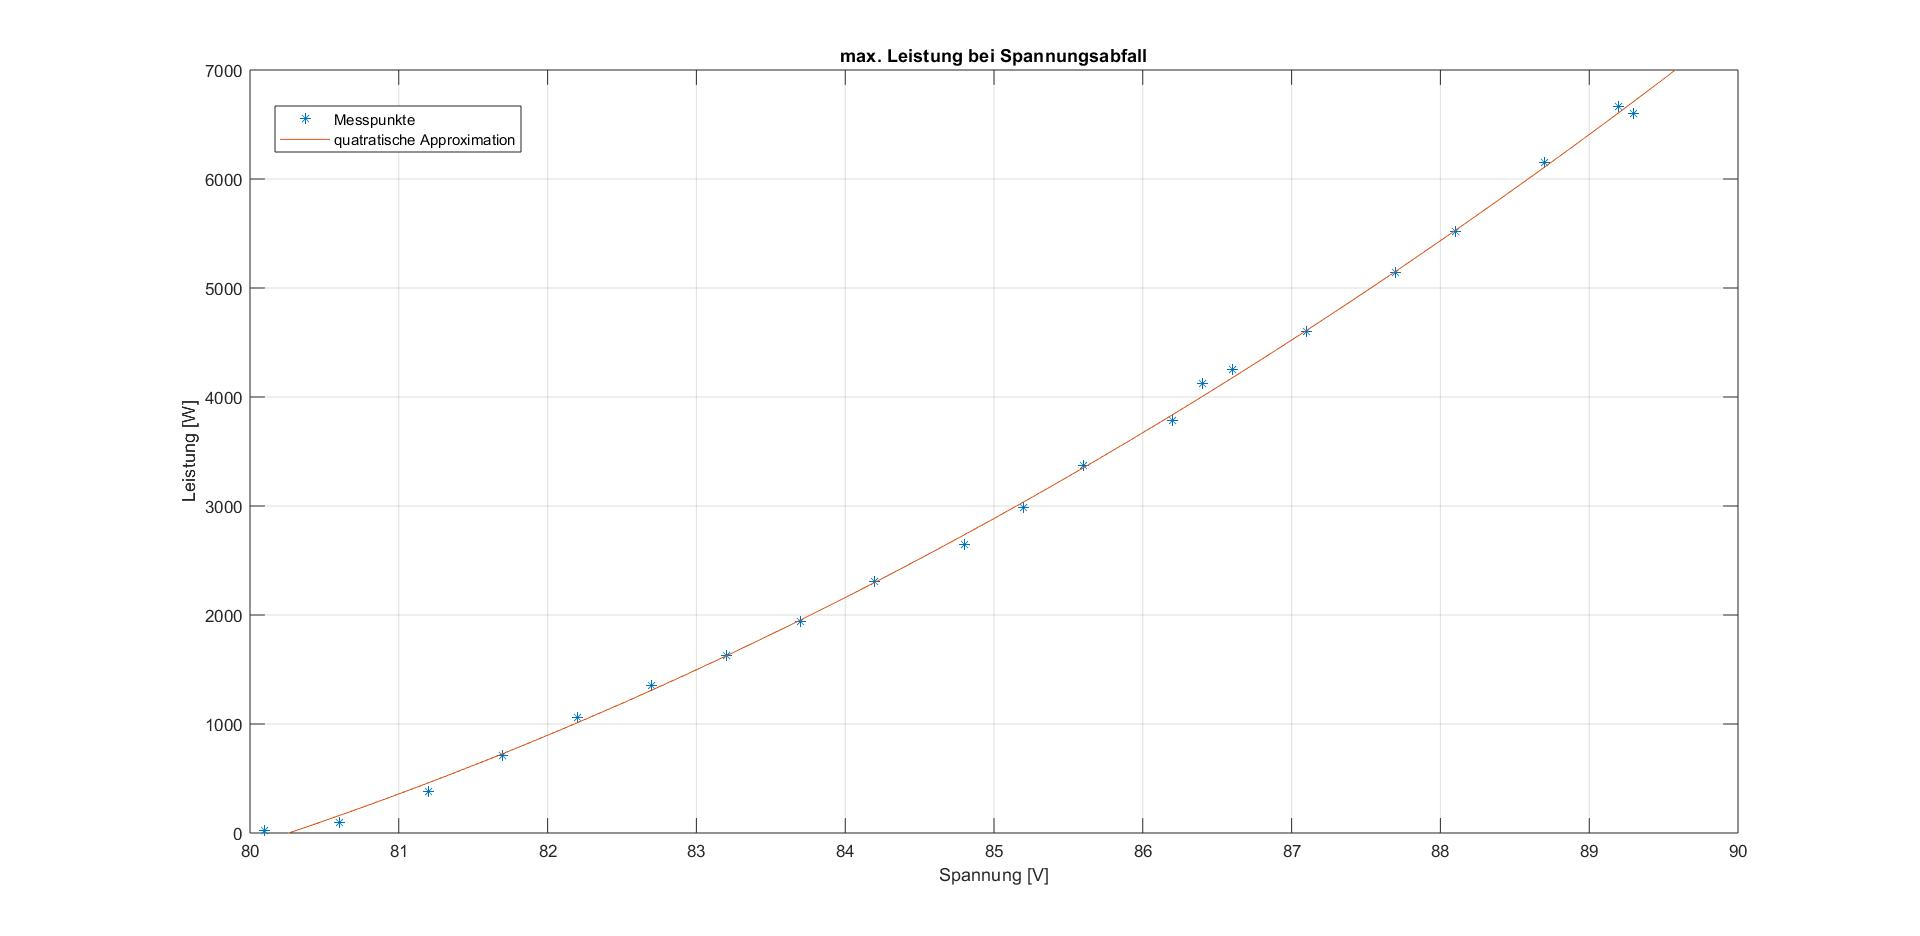
\includegraphics[width=0.8\linewidth]{maxLeistung.jpg}
	\caption{Maximale Leistung}\label{fig:maxLeistung}
\end{figure}

Unter der Annahme, dass zwischen der maximalen Leistung und der Spannung ein quadratischer Zusammenhang besteht, ist anzunehmen, dass die maximale Leistung bei 3600 RPM und Nennspannung (96V) bei 15kW liegt. Hierbei ist jedoch noch anzumerken, dass die effektive Leistung an der Welle ca. 10\% höher ist, da diese auf der elektrischen Seite der asynchronen Maschine gemessen wurde.

\subsection{Temperaturversuch}
In diesem Versuch wurden die Erwärmung in Abhängigkeit der Drehzahl bei konstantem Moment gemessen. Dabei wurde die Temperatur des BLDC-Motor bei 1550 RPM und bei 2550 RPM bei einem Drehmoment von 32Nm gemessen. Der Motor hatte am Anfang jeweils 60°C und wurde solang betrieben, bis er eine Betriebstemperatur von 100°C erreicht hat.


\begin{figure}[H]
	\centering
	\includegraphics[width=0.8\linewidth]{Temperatur.jpg}
	\caption{Erwärmung}\label{fig:Temperatur}
\end{figure}


Da bei gleichbleibendem Drehmoment aber höherer Drehzahl die Leistung höher ist, ist der Strom auch grösser. Dadurch ist die Erwärmung des Motors bei höheren Drehzahlen höher. Anhand der beiden Versuchen gehen wir davon aus, dass der BLDC-Motor ca. 5 Minuten unter Vollast betrieben werden kann, bis er die 100°C erreicht. Der Motor lässt jedoch eine Betriebstemperatur von 110°C zu, wodurch eine Reserve gegeben ist.
 